\section{Considerações Iniciais}

Neste capítulo pretende-se detalhar melhor o problema a ser resolvido. Posteriormente, será descrito todo o \textit{pipeline} de coleta e tratamentos dos dados para a montagem do conjunto de dados que será utilizado para treinamento e avaliação do modelo proposto.

\section{Detalhamento do Problema}

Ao chegar uma nova denúncia através do sistema FalaBR, da OGU, uma equipe de pessoas atua para avaliar as informações presentes na denúncia e decidir se a denúncia está apta a ser apurada ou não. Ou seja, a avaliação da equipe diz respeito a elementos presentes na denúncia que permitem uma apuração dos fatos relatados.

Em geral, estes elementos estão centrados em informações como CPF, CNPJ, Contratos e Convênios entre órgãos públicos e empresas privadas, materialidade (valores monetários descritos na denúncia ou identificados nos contratos e convênios). Com tais informações, a equipe de triagem de denúncias decide se deverá haver apuração (denúncia apta) ou não (denúncia não apta).

Uma grande parte deste trabalho pode ser automatizado. Assim, as consultas realizadas pela equipe, em diversos sistemas, podem ser substituídas por um processo automatizado, desde que seja possível identificar tais entidades no conteúdo das denúncias. Além disso, durante o processo de triagem, a equipe atribui uma nota de 0 a 100 (de 10 em 10) para definir o quão apta é uma denúncia. Por definições internas, notas entre 0 e 50 são consideradas não aptas e notas entre 60 e 100 são consideradas aptas. Tais notas podem ser utilizadas como rótulo para um aprendizado supervisionado.

Assim, sendo possível montar um conjunto de variáveis adequadas é possível propor a criação de um modelo para inferir notas às novas denúncias automaticamente.

O primeiro problema a ser resolvido, então, é a coleta e preparação dos dados. 
A próxima seção detalha os desafios enfrentados e como foram resolvidos.

\section{Coleta de Dados}

O processo de coleta e análise de dados para utilizar em treinamentos de aprendizado de máquina, geralmente, é composto por uma fase de análise exploratória. Em muitos casos, os dados estão estruturados e o maior trabalho é uma análise em que se verificam duplicidades, dados faltantes, \textit{outliers} e outras peculiaridades comuns em dados provenientes de sistemas informatizados. 
Já, no caso deste trabalho, não há, diretamente, dados estruturados. As únicas informações que podem ser obtidas são o texto da denúncia e os anexos, quando informados. Assim, a análise das denúncias e o seu uso para um aprendizado supervisionado devem abranger técnicas de NLP.

Como já foi mencionado, há rótulos sendo atribuídos às denúncias. Assim, o \textit{dataset} que será utilizado contém 1489 registros contendo informações da denúncia, anexos e a informação de grau de aptidão. Estes registros compreendem todas as denúncias cadastradas e que possuem rótulo atribuído entre 04/12/2019 e 23/06/2020.

\begin{figure}[htbp]
\caption{Quantidade de denúncias por rótulo}\label{fig_00100_quantidade_denuncias}
\begin{center}
    \includegraphics[width=\columnwidth]{images/fig_00100_quantidade_denuncias.png}
\end{center}
\legend{Fonte: Autor.}
\end{figure}

Conforme pode ser visto na \autoref{fig_00100_quantidade_denuncias}, a maior parte das denúncias recebeu um grau de aptidão 10, ou seja, são denúncias as quais os especialistas da OGU não possuem dúvidas de que as situações reportadas não devem ser apuradas.

\subsection{Extração de Textos dos Anexos}

Ao avaliar os anexos presentes em todas as denúncias cadastradas, identificou-se uma variedade muito grande de tipos de arquivos. Por essa razão, implementar um código, mesmo que utilizando bibliotecas prontas em Python \cite{rossum2009}, não se provou uma alternativa viável. Não foi possível identificar nenhuma biblioteca que conseguisse, sozinha, lidar com qualquer tipo de arquivo. Por outro lado, escrever um código para identificar o tipo de arquivo e realizar a chamada para uma biblioteca especializada no tipo de arquivo em questão não seria uma tarefa trivial e fugiria demais do escopo do trabalho.

Existe, no conjunto de dados avaliado por este trabalho, um total de 1801 anexos. A \autoref{fig_00050_quantidade_anexos_tipo_arquivo}, apresenta a quantidade de anexos de acordo com o tipo de arquivo.

\begin{figure}[htbp]
\caption{Quantidade de anexos por tipo de arquivo}
\label{fig_00050_quantidade_anexos_tipo_arquivo}
\begin{center}
\includegraphics[width=\columnwidth]{images/fig_00050_quantidade_anexos_tipo_arquivo.png}
\end{center}
\legend{Fonte: Autor.}
\end{figure}

Assim, para possibilitar a extração dos textos dos anexos, optou-se por utilizar uma ferramenta chamada Apache Tika (disponível em \url{http://tika.apache.org}) implementada em java. Esta ferramenta identifica automaticamente o tipo de arquivo e extrai o conteúdo textual e os metadados. A ferramenta, ainda, é capaz de realizar \sigla{OCR}{\textit{Optical Character Recognition}} quando há imagens dentro de arquivos dos tipo pdf, xls, doc, entre outros ou quando o arquivo é uma imagem.

Desta forma, configurou-se um servidor com a ferramenta instalada na forma de um serviço e utilizou-se uma biblioteca em Python para realizar as chamadas ao serviço passando os arquivos que deveriam ter o conteúdo extraído.

\subsection{Extração de Dados Estruturados}

A extração de dados estruturados é a tentativa de identificar certas entidades de interesse no conteúdo do texto da denúncia e seus anexos. As entidades de interesse, neste momento são CPF, CNPJ, convênios, contratos, NIS, nomes de pessoas, palavras fortes e valores.

Apesar de haver diversas formas de reconhecimento de entidades nomeadas, por questões de escopo e tempo, decidiu-se realizar a extração destas informações utilizando expressões regulares. A implementação de regras com expressões regulares para as entidades citadas acima, é simples na maioria dos casos e não exigem um treinamento como no caso dos algoritmos mencionados no \autoref{chapter:revisao_bibliografica}.

\subsection{Expansão das Informações}

Especialistas da OGU, ao analisar uma denúncia, pesquisam informações a partir do conteúdo das denúncias. Da mesma forma, a etapa de expansão compreende todos os dados estruturados, derivados daqueles encontrados na etapa anterior. 

Por exemplo, para um CPF citado, pode-se avaliar em quais CNPJs este CPF consta como sócio. Em um CNPJ pode-se avaliar os sócios. Em contratos ou convênios pode-se querer avaliar os participantes (órgãos e CNPJs), além do valor envolvido no ato administrativo. Para um nome de pessoa citado, pode-se tentar buscar o CPF caso não haja homônimos na base de CPFs da Receita Federal. Estas informações são extraídas e armazenadas mantendo-se a hierarquia, ou seja, um CNPJ extraído por que um CPF aparece no quadro societário possui um apontamento para o CPF que o originou e a relação ``é sócio de'' é preservada. Além disso, todos os dados estruturados preservam o identificador da denúncia a qual foram extraídos.

\begin{figure}[htbp]
    \caption{Exemplo de extração e expansão de dados estruturados}
    \label{fig_00200_extracao_expansao}
    \begin{center}
        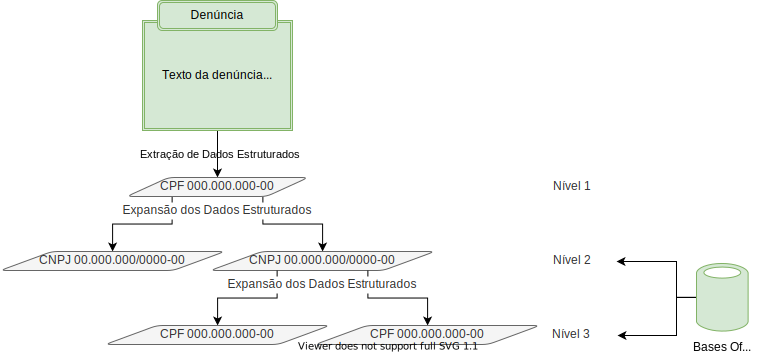
\includegraphics[width=\columnwidth]{images/fig_00200_extracao_expansao.png}
    \end{center}
\legend{Fonte: Autor.}
\end{figure}

A \autoref{fig_00200_extracao_expansao} apresenta um exemplo fictício no qual o processo de extração encontra um CPF. A partir deste CPF dois CNPJs, nos quais o CPF pertence ao quadro societário, são encontrados. Para cada CNPJ encontrado busca-se os CPFs dos demais sócios. Assim, os dados estruturados provenientes da extração são definidos como nível 1, seus dados estruturados derivados nível 2 e assim por diante. Avaliou-se que, acima do nível 3, a quantidade de dados estruturados aumentaria demasiadamente e os mesmos teriam pouca relevância. Assim, na base de dados utilizada para este trabalho serão expandidos e trabalhados apenas informações até o terceiro nível.

\subsection{Qualificação dos Dados Estruturados Encontrados}

O processo de qualificação tem por objetivo extrair outras características para cada dado estruturado encontrado, independentemente do nível. Assim, para um CPF encontrado, por exemplo, pode-se extrair informações como: é ou não servidor público federal, foi demitido da administração pública federal, possui processo administrativo disciplinar, é pessoa exposta politicamente, fez doações a partidos políticos (valor total das doações), entre outras. 

No caso de um CNPJ, como exemplo, podemos verificar se a empresa consta no \sigla{CADIN}{Cadastro Informativo de Créditos não Quitados do Setor Público Federal}, \sigla{CEPIM}{Cadastro de Entidades Privadas sem Fins Lucrativos}, se já teve outras sanções feitas pela administração pública federal, se a empresa fez doações a partidos políticos, entre outras.

As qualificações encontradas podem ser utilizadas como \textit{features} das denúncias.

\subsection{Preparação do \textit{Dataset}}

Esta etapa consiste na consolidação, em \textit{features} ou características, de todas as informações encontradas nas etapas anteriores. Assim, realiza-se um agrupamento por origem de informações. Algumas características como materialidade são somadas outras como CPF de servidor público são contabilizadas. Dessa forma, para cada denúncia, há um registro com uma quantidade grande de colunas nas quais consolidam-se todas as informações encontradas nas etapas anteriores. Por fim, inclui-se o rótulo. A \autoref{tab_00100_visao_geral_dataset} apresenta uma visão em alto nível de como o \textit{dataset} é montado bem como uma explicação da origem de algumas \textit{features} e sua forma de consolidação. 


\begin{table}[htbp]
\caption{Visão geral do dataset após o processamento das denúncias}
\label{tab_00100_visao_geral_dataset}
\tiny
\centering
\begin{tabular}{p{0.175\columnwidth}p{0.55\columnwidth}p{0.2\columnwidth}}
\toprule
     \textit{Feature} &
     Descrição &
     Forma de Consolidação \\
\midrule

    grau\_aptidao &
    Rótulo definido pelos especialistas &
    Único por denúncia \\
      
    txt\_denuncia &
    Conteúdo da denúncia &
    Único por denúncia \\
    
    txt\_anexos & 
    Conteúdo textual extraído dos anexos 
    &  Único por denúncia \\
    
    nome\_em\_denuncia 
    &  Nomes de pessoas encontrados no texto ou anexos da denúncia. São contabilizados apenas nomes existentes na tabela de pessoa física da receita federal
    & Contagem de ocorrências\\
    
    cpf\_em\_texto\_denuncia
    &  CPFs encontrados no texto ou anexos da denúncia
    & Contagem de ocorrências \\
    
    materialidade
    & Referências a valores monetários encontrados diretamente no texto da denúncia e seus anexos ou em contratos e convênios extraídos das mesmas
    & Soma dos valores \\
    
    denuncia\_anonima
    & Indicador se a denúncia é anônima ou não
    & Binário (1 ou 0) \\
    
    ... 
    &  ... 
    & ... \\
    
    palavras\_fortes
    &  Palavras fortes que possam levar ao entendimento de que há ato suspeito sendo denunciado (fraude, ilegal, desvio, superfaturamento, etc.)
    & Contagem de ocorrências \\
    
\bottomrule
\end{tabular}
\legend{Fonte: Autor.}
\end{table}%


Além das 7 \textit{features} e da variável alvo (rótulo) detalhadas na \autoref{tab_00100_visao_geral_dataset}, são extraídas outras 71 \textit{features}. O presente trabalho não detalhará as demais por questões de sigilo, considerando que a metodologia proposta será adotada na instituição em que o autor é vinculado.

Com o dataset finalizado pode-se iniciar a avaliação dos dados para a proposição de um modelo de classificação.